\documentclass[../../master_thesis_np.tex]{subfiles}
\graphicspath{{./imgs/}}

\begin{document}
\chapter[Interaction Implementation]{Implementation of interactions in simulations}
\label{chap:int_impl}

	All the code work in this thesis is built on top of an existing code written and used in Microscale Robotics Lab, which can be found in repository \cite{sharma_simulations_2023}.
    Existing code performed simulations on 2D active Brownian particles moving in open or closed boundary featuring confinement. 
	\todo{descrivi meglio il codice esistente: es. quali interazioni, quali condizioni al contorno, quali algoritmi di integrazione}
	
	\section{Simulation Framework}
	In order to simulate most physical systems, some fixed steps are needed and our case study makes no exception. 
	The main nodes of our simulation framework are:
	\begin{enumerate}
		\item Creation and preparation of all needed files
		\item Initialization of particle ensemble inside the simulation box
		\item Updating loop: a \verb|for| loop on time steps, which includes:
		\begin{enumerate}
			\item Force computation at time $n$, starting from positions at time $n$
			\item Generation of the needed random numbers for noise
			\item Integrator step: one step of the integration algorithm to get the ensemble at time $n+1$
			\item Application of boundary conditions and hard sphere correction 
			\item File writing of positions and orientations of all particles in ensemble \todo{ad ogni passo scrivi nel file?}
			\item Computation and file writing of global properties, e.g.\ polarization, pair correlation function etc.	\todo{questo ultimo step lo fai nel ciclo o fuori? non fa tanto parte della simulazione quanto dell'analisi}
		\end{enumerate}
		\item Files closing
		\item Plotting of necessary quantities, saving of animation for dynamics
	\end{enumerate}
	
	The main file that gets created at point 1.\ is the \emph{history} file, the one referred to in (d), to store positions and orientations of all particles. 
	It gets prepared as a comma spaced values (CSV) files, where the column names are written in advance. 
	CSV formatted files are more understandable and universally readable, which is useful when exchanging data between programming languages and manual checks are needed.
	\todo{magari spiega perché scrivi i dati in un file e non li mantieni in memoria, o fai riferimento a dove lo spieghi}
	
	In point 2.\ particles position are randomly initialized, with a uniform distribution in the simulation space. 
	We need to make sure that particles are not superimposed to avoid nonphysical effects. \todo{come lo fai?}
	At this point it is possible to compute forces and torques acting on every particle, which are needed to compute positions at the next step.
	
	From the computational point of view, our simulation framework is based upon object oriented programming: particle ensemble is initialized as an instance of the ABPE class, which holds all the variables that define the state of the system at a certain time \ref{tab:ABPE2}. 
	\begin{table}[h]
		\centering
		\begin{tabular}{c|cl}
			\textbf{Variable} & \textbf{Type} & \textbf{Description} \\
			\hline
			\texttt{Np}  & \texttt{Int64} & Number of particles \\
			\texttt{L}   & \texttt{Float64} & Size of observation space (\unit{\micro\meter}) \\
			\texttt{R}   & \texttt{Float64} & Particle radius (\unit{\micro\meter}) \\
			\texttt{T}   & \texttt{Float64} & Temperature (\unit{\kelvin}) \\
			\texttt{v}   & \texttt{Vector\{Float64\}} & Self-Propulsion Velocity (\unit{\micro\meter\per\second}) \\
			\texttt{$\mathtt{\omega}$}   & \texttt{Vector\{Float64\}} & Self-Propulsion Angular velocity (\unit{\radian\per\second}) \\
			$\mathtt{D_T}$  & \texttt{Float64} & Translational diffusion coefficient (\unit{\square\micro\meter\per\second}) \\
			$\mathtt{D_R}$  & \texttt{Float64} & Rotational diffusion coefficient (\unit{\square\radian\per\second}) \\
			\texttt{x}   & \texttt{Vector\{Float64\}} & Particle X position (\unit{\micro\meter}) \\
			\texttt{y}   & \texttt{Vector\{Float64\}} & Particle Y position (\unit{\micro\meter}) \\
			\texttt{$\mathtt{\theta}$}   & \texttt{Vector\{Float64\}} & Particle orientation (\unit{\radian}) \\
		\end{tabular}
		\caption{Structure definition of \texttt{ABPE} in Julia}
		\label{tab:ABPE2}
	\end{table}
	Global variables are numbers and all single particle variables, such as positions, are vectors of Np elements. %Some of variables are redundant, e.g.\ diffusion coefficients can be easily found starting from $T\text{ and } R$, as in \ref{eq:diff_coeff}, but it is useful to have them pre-computed for speed sake.
	\todo{attento al termine global variables, che potrebbe essere frainteso. Forse è meglio riferirsi a ensemble parameters o qualcosa del genere}
	
	In point 3.\ positions and orientations get updated with both the deterministic and stochastic parts of the dynamics. 
	This operation can be done either by updating a single instance of ABPE class or by appending to a pre-allocated vector one instance for every time step. 
	The first method is more memory efficient, and it is the one to prefer if no memory is needed, i.e.\ only step $n$ counts to determine what happens at step $n+1$. 
	A minimal example of this workflow, with Euler as an integrator\todo{mi immagino il vecchio Eulero lì a integrare a mano... scrivila meglio}, is in algorithm \ref{alg:sim1}.
	
	\begin{algorithm}
		\caption{The simulation algorithm} \label{alg:sim1}	
		\begin{algorithmic}[1]
			\For{$i$ in $[1,\mathtt{Np}]$}
			\State{$ \vec{r}_{i}\gets \vec{r}_{i,0} $}\Comment{position $\vec{r}_{i,0}$ is randomly initialized in the simulation space}
			\State{$\theta_{i}\gets \theta_{i,0}$}\Comment {$\theta_{i,0} \sim \mathrm{Uniform}([0, 2\pi])$}
			\State{$v\gets v_0$}\Comment{Can be initialized as a constant or a random variable}
			\EndFor
			\For{n in timesteps}
			\For{$i$ in $[1,\mathtt{Np}]$}
			\State{$\vec{F}_{i,n} = \sum_{j \neq i}^{Np}{\vec{F}_{ij,n}}$}
			\State{$w_{i,n} \sim \mathcal{N}(0, \sqrt{2D_t \Delta t})$}
			\State{$z_{i,n} \sim \mathcal{N}(0, \sqrt{2D_r \Delta t})$}
			\State{$ \vec{r}_{i,n+1}\gets \vec{r_n} + w_{i,n} + v (\cos\theta_{i,n}, \sin\theta_{i,n})\Delta t + \vec{F}_{i,n}\Delta t D_t/k_B T $}
			\State{$\theta_{i,n+1}\gets \theta_{i,n} + z_{i,n} + \omega_{i,n} \Delta t + M_{i,n} \Delta t D_r/k_B T$}
			\EndFor
			\EndFor
		\end{algorithmic}
	\end{algorithm}  
	
	\section{Methods}
	All the simulation and analysis code for this thesis was written in \julia\ \cite{julia}\todo{carino, ma un po' piccolo}, except for the machine learning and inference part, where the Graph Network definition and training makes use of Python libraries like PyTorch \cite{pytorch} and PyTorch-geometric \cite{pyg}, along with standard scientific computing tools like NumPy \cite{numpy} and Pandas \cite{pandas}.
	
	{\color{brown}The Heun algorithm} was chosen as the standard integration scheme for all the simulations, and integration steps vary with the different potentials and are indicated case by case. 
	All the simulations were performed with real units, so that particles have a radius of \SI{2}{\um} and the value for solvent viscosity is kept fixed at \SI{1e-3}{\pascal\second}. 
	If not indicated, standard temperature for simulations is held fixed at \SI{300}{\kelvin}.
	
	All simulations were performed in a two-dimensional square environment, where particles are disks, featuring periodic boundary conditions and a non-superposition condition (hard sphere correction). 
	Given that positions are simulated in open periodic boundary, all interactions are calculated periodically too, taking the shortest between the in-box and the periodic distance.
	
		\section{Boundary Conditions and Hard Sphere Correction}
	%\todo{tutta questa sezione la sposterei prima di quella precedente, visto che l'implementazione delle interazioni è il contributo principale di questo lavoro}
	\subsection{Boundary Conditions}
	Original code featured open, periodic or hard boundary conditions. 
	We will not go through all of them, but briefly, open boundary conditions means letting particles free to move out the simulation box, which in this case becomes just an \emph{observation space}, while a hard wall involves computing boundary's gradient in any point and using it as a locally straight wall condition.
	
	Periodic boundary conditions for a square simulation area are straightforward to make work if one places the origin in the center of the square. 
	Then, if $L$ is square's side, limits for particles' motion will be $\pm L/2$ in both axes. 
	The actual limit for them to be reflected is $L/2 + R$, meaning a particle must be entirely sticking out before being moved to the other side. %\todo{questo alla fine lo abbiamo lasciato così?}
	These physical boundary conditions are implemented according to algorithm \ref{alg:pbc}.
	
	\begin{algorithm}[htp]
		\caption{Periodic Boundary Conditions} \label{alg:pbc}	
		\begin{algorithmic}[1]
			\ForAll{positions $(x,y)_i$}
			\If{$\abs{x_i} > L/2 + R$}\Comment{$R$ is the particles' radius, $L$ box side}
			\State{$x_i \gets x_i - \mathrm{sign}(x_i)L$}
			\EndIf
			\If{$\abs{y_i} > L/2 + R$}\Comment{$R$ is the particles' radius, $L$ box side}
			\State{$y_i \gets y_i - \mathrm{sign}(y_i)L$}
			\EndIf
			\EndFor
		\end{algorithmic}
	\end{algorithm}
	
	\subsection{Hard Sphere Correction}
	\label{hs}
	Original simulation code featured just steric hard sphere correction as interactions among particles, which are enough to study clustering, MIPS and boundary accumulation.
	The hard sphere correction follows algorithm \ref{alg:hardsphere} according to \cite{callegari_numerical_2019}.
	
	\begin{algorithm}[htp]
		\caption{The hard sphere correction algorithm} \label{alg:hardsphere}	
		\begin{algorithmic}[1]
			\ForAll{couples of particles $\{i, j\}$}
			\State{$d_{i,j} \gets d(\mathbf{r}_{i}, \mathbf{r}_{j})$} \Comment{$d\left(\cdot,\cdot \right)$ is the Euclidean distance}
			
			\State{$\mathbf{n}_{i,j} = \left(\mathbf{r}_{i}-\mathbf{r}_{j}\right)/d_{i,j}$}
			\If{$d_{i,j} < 2R$}\Comment{$R$ is the particles' radius}
			\State{$\mathbf{r}_i \gets \mathbf{r}_i - \mathbf{n}_{i,j}d_{i,j}/2$}
			\State{$\mathbf{r}_j \gets \mathbf{r}_i - \mathbf{n}_{j,i}d_{i,j}/2$}
			\EndIf
			\EndFor
		\end{algorithmic}
	\end{algorithm}
	
	\begin{figure}[htp]
		\centering
		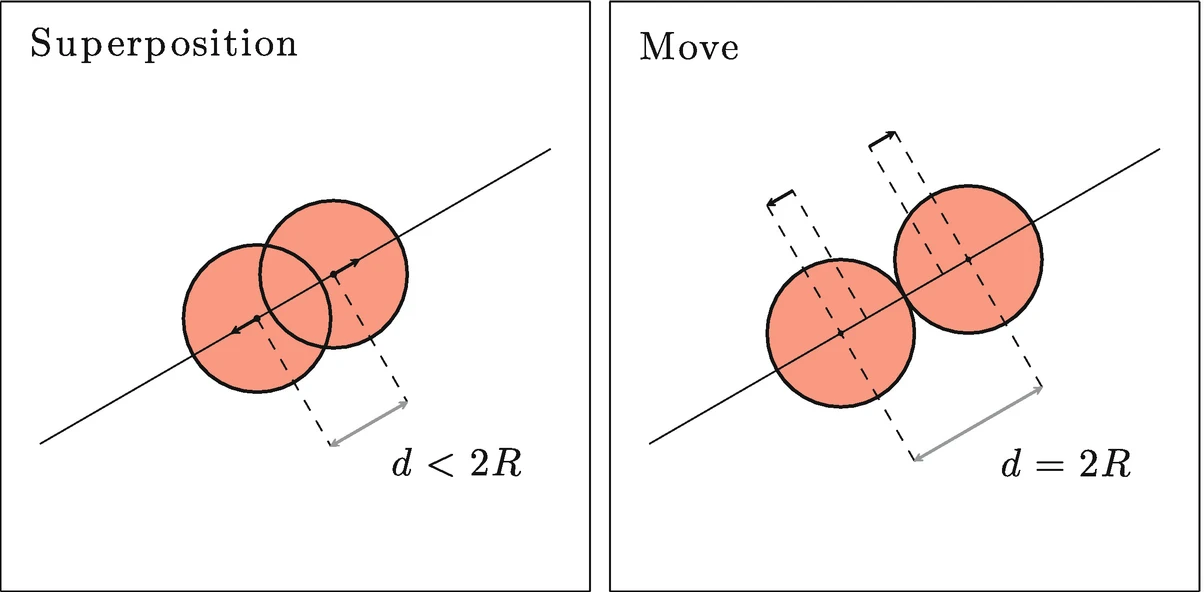
\includegraphics[width = \textwidth]{callegari_volpe_2019_hardsphere.png}
		\label{fig:hardsphere}
		\caption{If in one step two particles superimpose, hard sphere correction moves them at one diameter distance \cite{callegari_numerical_2019}}
	\end{figure}
	
	This operation involves calculating the distance matrix of a set of $\mathtt{N_p}$ particles, i.e.\ computing $\mathtt{N_p}^2$ distances.
	Being a $\order{n^2}$ algorithm, this kind of correction can become computationally demanding, especially for high density and velocity systems, where collisions and clustering are more likely to happen. 
	Moreover, correction showed in algorithm \ref{alg:hardsphere} is for only one step and it does not guarantee zero superposition afterwards.
	It becomes important to let the algorithm have a small tolerance, like $1/1000$ of particle radius and to cycle the correction until the number of superposition becomes zero.
	
	In the work cited in section \ref{literature}, \citeauthor{martin-gomez_collective_2018} use a steep repulsive potential $\sim r^{-12}$ to simulate the excluded volume.
	In principle, since it does not require cycling, this approach seems faster, especially if one has to compute interactions.
	During the development of this thesis some tests were run and, with all integration algorithms, even though computing the excluded volume effect is actually faster than applying a hard sphere correction, the steep potentials involved require a much smaller time step (1 or 2 orders of magnitude), making the simulation slower.
	
	Separating superimposing particles in a way to keep them in contact may seem a strong assumption, since it is simulating a perfectly inelastic collision.
	This choice arise due to the finite contact time and micron sized physics of the active particles under study.
	In macroscopic Newtonian dynamics scenario (balls moving on a pool table), it is relatively easy to state collisions' elastic or inelastic nature.
	Furthermore, in the Microscale Robotics Lab and in literature \cite{singh_pair_2024}, Janus active particles collisions are observed to have a finite contact time $\sim\SI{}{\second}$.
	This long collision time encouraged us to implement inelastic collision in simulations.
	
	\subsection{Modified Periodic Boundary Steric Interactions}
	Since hard-sphere corrections were implemented to study ABPs in confinement rather than open periodic boundary, this interaction could not take periodicity into account leading to possible superpositions at boundaries.
	
	When boundary conditions are periodic, not taking them into account in steric interactions may cause some problems, on top of being not formally correct.
	With the hard-sphere correction as it was described in section \ref{hs}, particles are separated when their distance is less than their diameter.
	With periodic boundary conditions, a particles is reflected {\it e.g.}, on the left hand side only when its center is out of the right hand side by more than one particle radius ($R$).
	This may leave a \emph{frame} of size $R$ around the boundary where inter-particle periodic distance can be less then $2R$. 
	
	When combined with potentials that feature a \emph{soft} non-superposition condition, like a diverging positive force at a $2R$ distance, this can lead to pairs of particles sticking out of the border on opposite sides and superimposing a lot before one of them gets reflected on the other side, but when this happens, the force between them diverges, resulting in nonphysical situations like particles moving far outside the box.
	
	To address this issue, we propose a modified version of hard sphere corrections where distances are not computed in a Euclidean fashion, but $x$ and $y$ components are separately checked.
	For a box of size $L$, we compute $\Delta x = min \left\{ \abs{x_1-x_2}, \abs{x_1-x_2}-L \right\}$, and the same for $y$, which is the right periodic distance between any given pair of particles.
	If $\Delta x < 2R$, particles are guaranteed to superimpose when periodic boundary condition is applied.
	To eliminate this superposition, we implemented the hard sphere correction as in section \ref{hs} to superimposing pairs at the boundary.
	This method allows us to identify superpositions at the boundaries, thus giving the possibility to form clusters starting from a \emph{nucleation site} on the border. 
	
	\begin{figure}[htp]
		\centering
		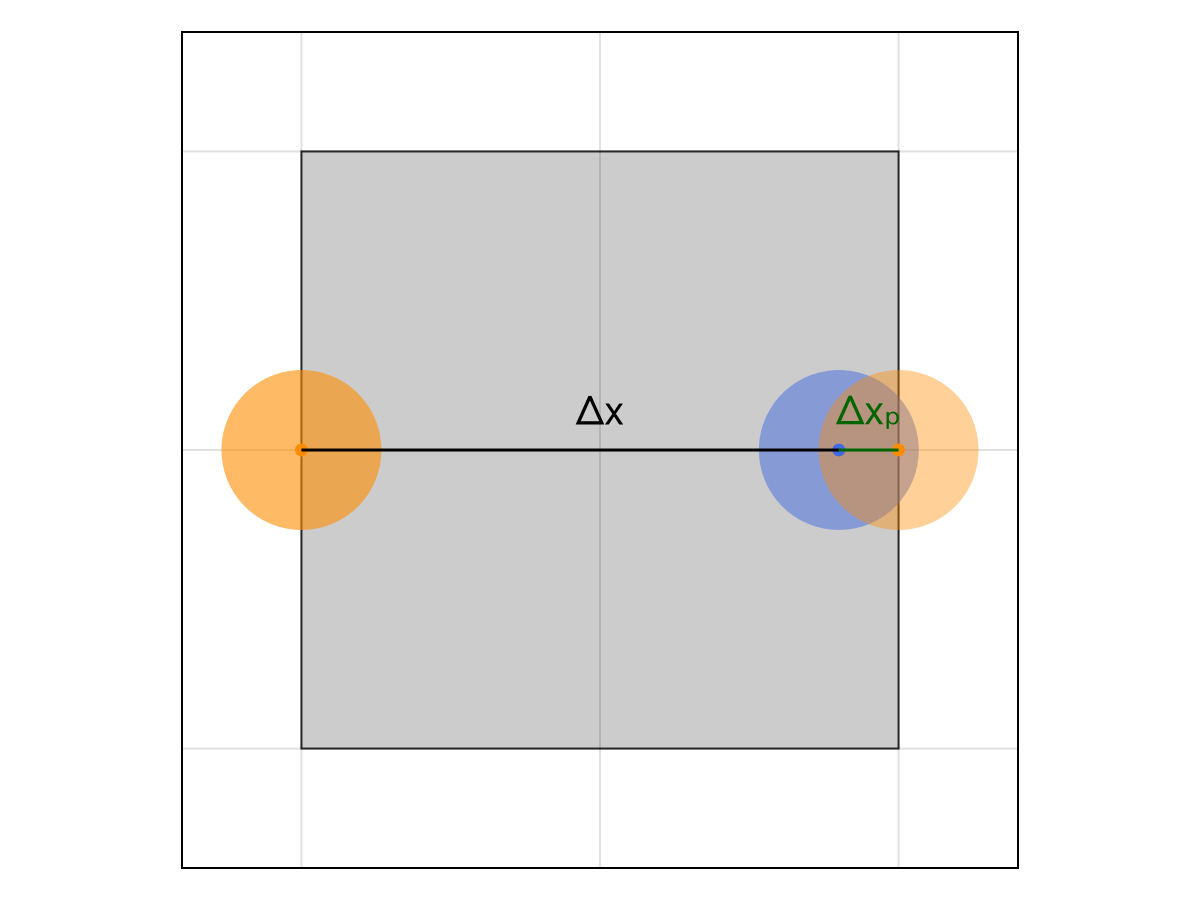
\includegraphics[width = \textwidth]{periodic_hs.png}
		\label{fig:periodic_hs}
		\caption{Orange particle is sticking out on the left side. Its \emph{real} distance from blue particle on x-axis is $\Delta x$. Its periodic projection (faded orange) has a distance from blue particle $\Delta x_p < 2R$, hence superimposing.}
	\end{figure}

	\section{Interaction Forces}
	
	\subsection{Central Potentials}
	%\todo{non capisco questo titolo... in che senso all to all?}

	Spring, Coulomb, Lennard Jones, Yukawa, Weeks-Chandler-Anderson are just few examples of the myriad of central potentials that are used to model interactions in physics. 
	The central potential is the basis of this thesis too, and having a fast implementation is crucial to simulate interactions in dense systems. 
	
	The first step {\color{brown}to apply a potential} is to compute a distance matrix between the coordinates of all particles. 
	Then a function $F(d)$, only of inter-particle distance $d$, is applied to all the entries of this matrix to get the magnitude of the force between each pair of particles. 
	In 2D, radial direction for the force can be computed from distance matrices both for $x$ and $y$ coordinates. 
	If $d^x_{i,j} = x_i - x_j$ and $d^y_{i,j} = y_i - y_j$, then Euclidean distance is $d_{i,j} = \sqrt{(d^x_{i,j})^2 + (d^y_{i,j})^2}$, and if $\varphi_{i,j}$ is the radial direction from particle $i$ to particle $j$, then
	\begin{equation}
		\begin{cases}
			\cos\varphi_{i,j} = d^x_{i,j}/d_{i,j}\\
			\sin\varphi_{i,j} = d^y_{i,j}/d_{i,j}
		\end{cases}
	\end{equation}
	splitting the force in its two components.
	Now the computed force can be used to calculate the deterministic step in the coordinate as in algorithm \ref{alg:sim1}: given that we are in low Reynolds number regime, \emph{velocity} is proportional to force . 
	%\todo{non chiaro... sembra che sommi delle forze a delle posizioni}
	
	\subsection{Tested Potentials}
			
	We give here the expressions and parameters explanation for the potentials tested in this thesis.
	%\todo{perché hai scelto questi potenziali?}
	
	\subsubsection{Spring potential}
	We used this potential to test a strong long-range interaction between particles, with some control over the equilibrium position.
	Spring force has two parameters, elastic constant $k_S$ and rest length $r_0$, so that 
	\begin{equation}
		V(r) = \frac{1}{2}k_S (r-r_0)^2 \rightarrow F(r) = -k_S(r-r_0).
	\end{equation}
	%\todo{dì qualcosa su questo potenziale, es. per cosa può essere usato, se è tipicamente short range o long range, etc.}
	%\todo{visto che usavi $k$ per entrambi i potenziali, forse sarebbe meglio usare $k_S$ per la costante elastica e $k_C$ per la costante coulombiana}

	\subsubsection{Coulomb potential}
	What we will often call Coulomb force is actually a $r^-2$ order potential with a constant $k_C$ that does not involve charges and it is present only to adjust the strength of interaction, that writes
	\begin{equation}
		V(r) = -\frac{k_C}{r} \rightarrow F(r) = \frac{k_C}{r^2}
	\end{equation} 
	and any sign variation, as well as the difference between repulsive and attractive, is absorbed in $k_C$.
	Being an attractive or repulsive-only potential, it can be used to study the effect of a potential in a relatively simple situation, especially when dealing with aligning interactions.
	Its divergence is not so steep thus letting us utilize larger integration steps.
	%\todo{dì qualcosa su questo potenziale, es. per cosa può essere usato, se è tipicamente short range o long range, etc.}

	\subsubsection{Lennard Jones potential}
	The last interaction potential is Lennard Jones (LJ)
	\begin{equation}
		V(r) = 4\varepsilon \left[ \left(\frac{\sigma}{r}\right)^{12} - \left(\frac{\sigma}{r}\right)^{6} \right] \rightarrow F(r) = 24\varepsilon \frac{1}{r}\left[ 2 \left(\frac{\sigma}{r}\right)^{12}  - \left(\frac{\sigma}{r}\right)^{6} \right]
	\end{equation}
	where $\sigma$ is a location parameter that in our simulations will be fixed at the value of particle's diameter $2R$, and $\varepsilon$ adjusts the strength of interaction. 
	This potential has an absolute minimum for $r = 2^{1/6}\sigma$.
	LJ is a standard in molecular dynamics and disordered systems, both its original version and its variations are often used in ABP research, since this potential encloses both short range repulsion to avoid superpositions and medium range attraction to give structure to the system.
	The short range divergence is pretty steep and its strong non-linearity requires very short integration times, better if coupled with advanced integration algorithms.
	%\todo{dì qualcosa su questo potenziale, es. per cosa può essere usato, se è tipicamente short range o long range, etc.}
	
	\begin{figure}[htp]
		\centering
		\subfloat[][]{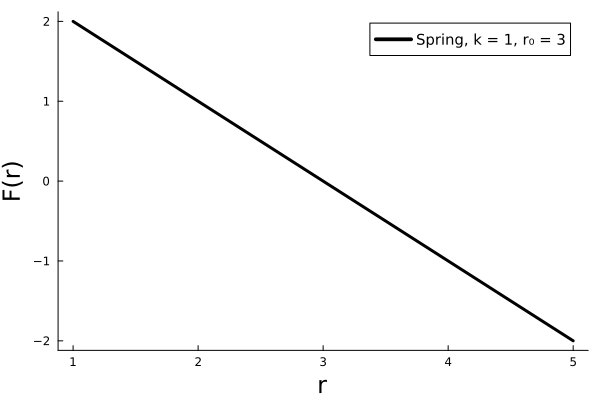
\includegraphics[width=\subfigwidth]{spring.png}}\quad
		\subfloat[][]{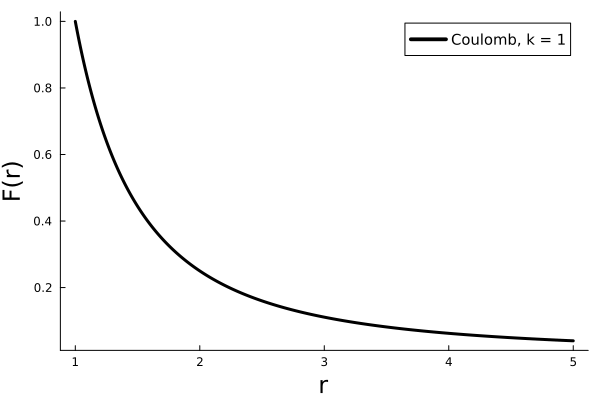
\includegraphics[width=\subfigwidth]{coulomb.png}}\quad
		\subfloat[][]{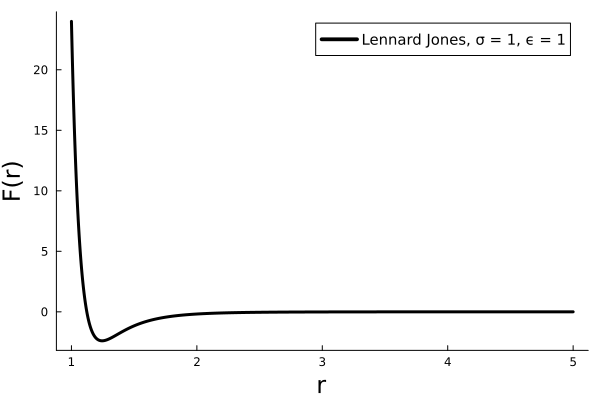
\includegraphics[width=\subfigwidth]{lj.png}}
		\caption{Tested interaction forces for given values of their parameters.}
		\label{fig:potentials}
	\end{figure}
	\todo{figura dei 3 potenziali un po' piccola (soprattutto il testo), e forse sarebbe meglio mettere le tre curve nello stesso grafico (se resci a dargli range di forze simile)}
	
	\todo{perché le figure de grafici in png e non in pdf / svg  o altri formati vettoriali?}
	\todo{è vero che abbiamo detto che i grafici sono più belli senza griglia, ma sarebbe utile avere almeno una linea orizzontale a zero, o spostare l'asse orizzontale in modo che passi per zero}
		
	\subsection{Interaction Range} \label{intrange}
	In some situations is useful to have a way to restrict the force computation only to particles closer than a threshold distance.
		
	One could do this to imitate a topological interaction at short range, where a particle only interacts with its nearest neighbors. 
	In the case of circular particles (or spherical in 3D), setting the range to $3R$ is enough to get this effect, since two particles in contact will have their centers at $2R$ and no other particle can be at less than $3R$ in the same directions. 
	This way, central particle will interact with 6 other particles at most (this is the number of nearest neighbors for hexagonal close packing order 2D) giving the effect of a nearest neighbor interaction in the case of contact. 
	Clearly, this is not a \emph{true} topological interaction, where two nearest neighbors interact regardless {\color{brown}of} their distance, but it can give similar effects if applied in high packing fraction cases, where particles come in contact.
	
	{\color{brown}Moreover, when dealing with fast decreasing potentials, the magnitude of the force between two distant particles can be effectively negligible and even lower than the numerical precision.}
	If this is the case, it is obviously pointless to look into pairs of particles which are more than a certain distance apart. 
	One can compute this distance for any given potential, provided some reference magnitude. 
	An example is given in Figure \ref{fig:force_zero}.
	\begin{figure}[htp]
		\centering
		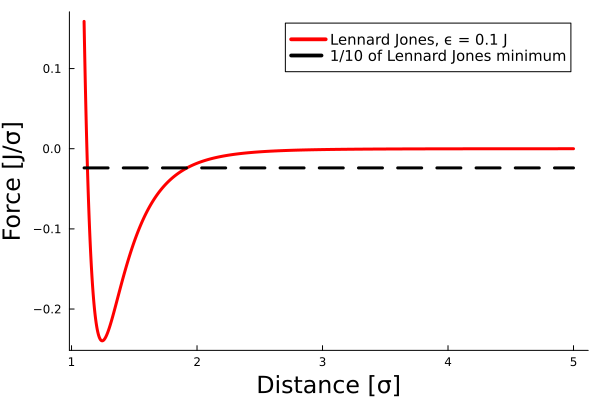
\includegraphics[width=\textwidth]{lj_zero.png}
		\caption{Cutoff for Lennard Jones force at $1/10$ of the minimum. The cutoff distance is $\sim 1.9\sigma$}
		\label{fig:force_zero}
	\end{figure}
	\todo{se confronti la dimensione del font di questa figura (cutoff) con quello della figura precedente (potenziali), noterai che sono diversi. sarebbe meglio uniformarli, come discutevamo l'altro giorno}
	This is of paramount importance for speed. 
	While a complete calculation of all the possible forces between $n$ particles is an $\order{n^2}$ algorithm (the actual number of possible interactions is $n(n-1)$), the number of particles in a box of given area is constant in $n$ if density remains fixed, so, scaling up the number of particles in the same conditions will be less demanding in terms of computational power.
	
	Inserting a range in interactions makes straightforward to apply them in a periodic fashion. 
	Though interactions were not featured in original code, functions for boundary conditions were implemented in a fast vectorized way, letting us reuse the existing function to reflect particles in periodic boundary conditions (pseudo code in algorithm \ref{alg:pbc}) in the interactions part. 
	%\todo{collega meglio queste due frasi, altrimenti sembra che la periodicità nell'interaction range fosse già presente nel codice originale}
	The idea is: take one particle and make it the \emph{central} one, then shift coordinates of the other particles so that the \emph{central} is in $(0,0)$, now just apply periodic boundary conditions to the shifted coordinates.
	This process should guarantee that the \emph{central} particle interacts only once with any of the others, following a simple rule: when choosing between the true particle and the periodically shifted one the interacting particle is the closest one.
	An explanation of this process can be found in Figure \ref{fig:periodicint}.
	
	\begin{figure}[htp]
		\centering
		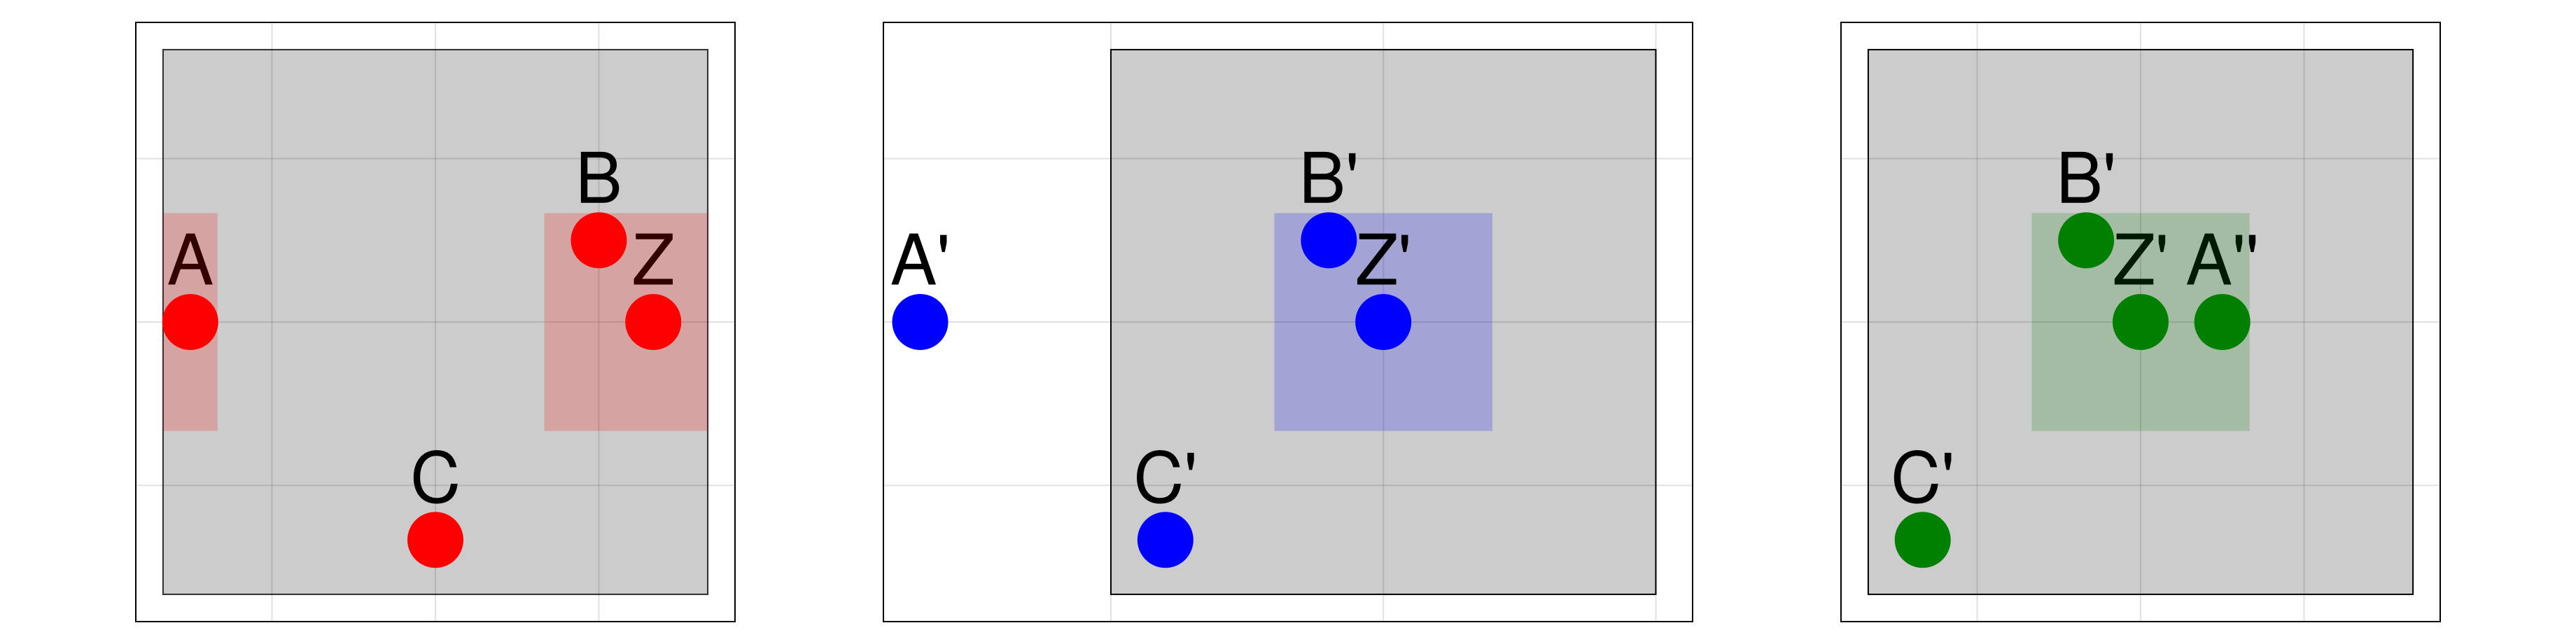
\includegraphics[width=\textwidth]{periodic_interaction.png}
		\caption{Red: original points with Z as central point and its interaction box sticking out on the opposite side. Blue: shifted points w.r.t.\ Z. Green: shifted points with PBC applied.}
		\label{fig:periodicint}
	\end{figure}
	
	\todo{i numeri sugli assi della figura su periodic interaction sono illeggibili}

	\subsection{Aligning Interactions} \label{alignint}

	There are several examples in literature of aligning interactions applied to ABPs systems \cite{martin-gomez_collective_2018, callegari_numerical_2019}.
	Most of them involve applying a torque which explicitly depends on the difference between the orientation angle of the two interacting particles; some of them have a constant torque which is applied to particles closer than a certain distance.
	{\color{brown}To the best of our knowledge, nobody have implemented interactions in a way that unifies the central force interactions and the aligning interactions.}
	
	The model used in this thesis aims to keep a minimal amount of parameters while coupling positions and orientations of interacting particles, actually using only one more parameter than a force-only model.
	{\color{brown}When applying a central potential interaction to a set of particles, the distances $r$ between particles are calculated with respect to the particles' centers and the computed interaction force $F^i(r)$ is applied to the particles centers as $\left[F^i_x\, F^i_y\right]$ (2D simulations).}
	Here every particle is identified by two positions: its center of mass, which lies in its geometric center, and an interaction center, which is translated with respect to the center of mass of an amount $\alpha R$ in the direction of self-propulsion, so that the off center position of each particle writes:
	\begin{equation}
		\vec{x}_{oc} = \vec{x}_{c} + \alpha R 
		\begin{pmatrix}
			\cos(\theta)\\
			\sin(\theta)
		\end{pmatrix}
	\end{equation}
	%\todo{ho messo $\vec{x}_{c}$ invece di $\vec{x}_{cm}$ perché mi sembrava che cm richiamasse centimetri}
	where $\theta$ is the self-propulsion direction, $R$ is the particle's radius, and $-1 < \alpha < 1$. 
	{\color{green}Compared to the self-propulsion direction, the off-center position is on the front half of the particle when $\alpha > 0$ and on the back half when $\alpha < 0$.}
	{\color{brown}Distances, and hence forces, are thus computed between the off-center positions. 
	Applying forces off center results also in an effective torque applied to the particle, leading to both translational (repulsive/attractive) and rotational (aligning) effects, coupling the two degrees of freedom.}
	\todo{possiamo effettivamente parlare di degrees of freedom in questo contesto?}
	
	The idea is to take into account the underlying particle's asymmetry not only in terms of self-propulsion but also in terms of interactions. 
	It is a fact that the two faces of a Janus particle have different physical and chemical properties, which make them interact differently depending on the angle between their orientations and the line connecting their centers \cite{singh_pair_2024}. 
	{\color{brown}This can be due to a plethora of effects like chemical gradients, electrical forces, hydrodynamics or fabrication defects that would be hard to model in details and effectively impossible to simulate for even a few particles.
	This model takes only the asymmetry and uses it along with standard potentials, to create a minimal dry framework that mimics such a complex wet dynamics.} 
	In doing so, we also show that this model displays some interesting statistical mechanics properties.
	
	\begin{figure}[htp]
		\centering
		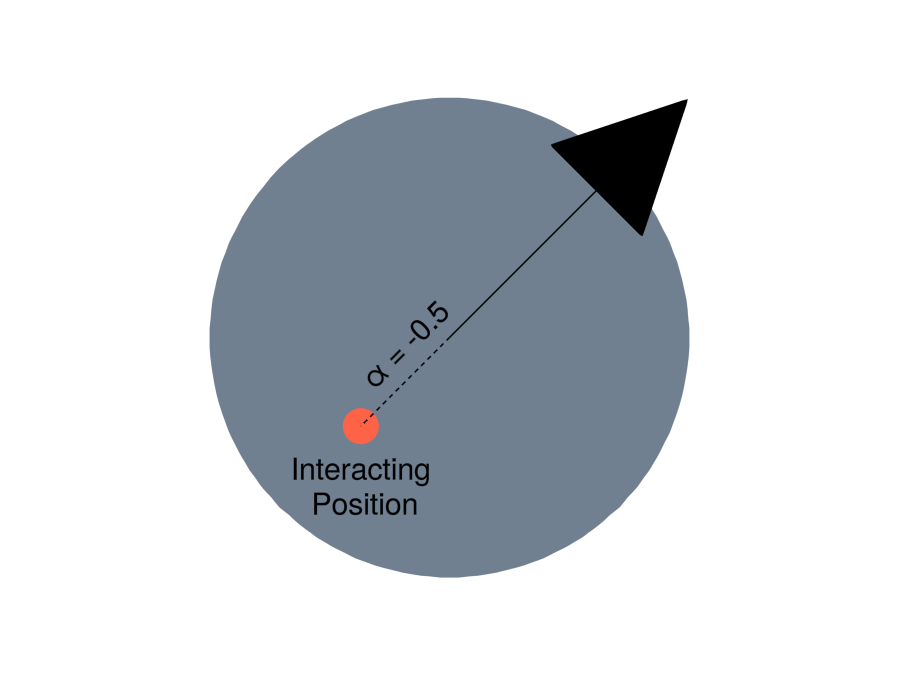
\includegraphics[width=\textwidth]{singpart_draw.png}
		\caption{\color{brown}Red point: position from which interaction distances are calculated and to which force is applied. In this case, interacting position is at $-0.5R$ from particle's center, {\it i.e.}\ on the back side compared to  the direction of self propulsion.}
		\label{fig:geom_model}
	\end{figure}
	
	{\color{green}\section{Results}}
	\todo{questa sezione dovrebbe contenere più in generale esempi di simulazioni e in particolare confronti con esperimenti}
	{\color{brown}\subsection{Qualitative comparison between experiments and simulations}} \label{qualitative}
	
	

\end{document}